%---------- Inleiding ---------------------------------------------------------

\section{Introductie}%
\label{sec:introductie}

Je hebt waarschijnlijk de reclame over de Metaverse `The Impact Will Be Real` van \textcite{Meta2022} gezien. Daarin tonen ze hun visie over de rol die Virtual Reality (VR) speelt in de toekomst. Zo laten ze verschillende toepassingen ervan in het onderwijs zien. Jammer genoeg staat onze technologie nog niet zo ver als wat er in de reclame gezien kan worden maar ook nu al vind VR zich een baan in verschillende opleidingen.

De Hogeschool van Gent maakt ook gebruik van VR om studenten de kans te geven in meer realistische situaties te oefenen. Hiervoor zijn twee verschillende technieken gebruikt. Allereerst heb je het renderen van een omgeving. Dit laat de gebruiker een interactieve wereld van 3D modellen ontdekken. Zo bestaan er drie virtuele kamers waarin de student kan oefenen. De andere manier is aan de hand van een 360° opname die wordt gemaakt aan de hand van een 360° camera. Omdat dit een opname van de werkelijkheid neemt, ziet deze methode er realistischer uit.

Dit is waar er op het probleem wordt gestoten. Aangezien de tweede methode werkt met een opname moet er naar verschillende fragmenten gesprongen worden naar gelang het antwoord dat de gebruiker ingeeft. Dit wordt handmatig gedaan via een meerkeuzevraag wat de immersie van de VR weg haalt. Daarom wordt in deze bachelorproef toegepaste informatica onderzocht hoe het overschakelen anders kan aangepakt worden zodat het voor de gebruiker realistischer aan voelt. Hiervoor kijken we richting Artificiële Intelligentie (AI).

Alle grote IT bedrijven hebben wel een departement die zich bezig houdt met AI. Ze zien allemaal de mogelijkheden die het biedt. Van jobs gemakkelijker te maken tot het zelf creëren van kunst, de toepassingen zijn oneindig. Daarom zal in functie van het zorglab op zoek worden gegaan naar een Spraak naar tekst (STT) en een natuurlijke taalverwerking software (NLP).

De STT zal worden gebruikt om het manueel ingeven van het antwoord te vervangen. In plaats daarvan zal de gebruiker gewoon zijn antwoord luidop kunnen geven en zal de STT dit in tekst omzetten. Dit alleen zal natuurlijk geen volgend fragment voor de gebruiker kunnen kiezen en daarom hebben we de NLP nodig. Deze zal de gegenereerde tekst omzetten naar kernwoorden en aan de hand daarvan bepalen welk fragment als volgende geschikt is.



% Waarover zal je bachelorproef gaan? Introduceer het thema en zorg dat volgende zaken zeker duidelijk aanwezig zijn:
%
%\begin{itemize}
%  \item kaderen thema
%  \item de doelgroep
%  \item de probleemstelling en (centrale) onderzoeksvraag
%  \item de onderzoeksdoelstelling
%\end{itemize}
%
%Denk er aan: een typische bachelorproef is \textit{toegepast onderzoek}, wat betekent dat je start vanuit een concrete probleemsituatie in bedrijfscontext, een \textbf{casus}. Het is belangrijk om je onderwerp goed af te bakenen: je gaat voor die \textit{ene specifieke probleemsituatie} op zoek naar een goede oplossing, op basis van de huidige kennis in het vakgebied.
%
%De doelgroep moet ook concreet en duidelijk zijn, dus geen algemene of vaag gedefinieerde groepen zoals \emph{bedrijven}, \emph{developers}, \emph{Vlamingen}, enz. Je richt je in elk geval op it-professionals, een bachelorproef is geen populariserende tekst. Eén specifiek bedrijf (die te maken hebben met een concrete probleemsituatie) is dus beter dan \emph{bedrijven} in het algemeen.
%
%Formuleer duidelijk de onderzoeksvraag! De begeleiders lezen nog steeds te veel voorstellen waarin we geen onderzoeksvraag terugvinden.
%
%Schrijf ook iets over de doelstelling. Wat zie je als het concrete eindresultaat van je onderzoek, naast de uitgeschreven scriptie? Is het een proof-of-concept, een rapport met aanbevelingen, \ldots Met welk eindresultaat kan je je bachelorproef als een succes beschouwen?

%---------- Stand van zaken ---------------------------------------------------

\section{State-of-the-art}%
\label{sec:state-of-the-art}

Om de immersie in de simulatie te vergroten moet ervoor gezorgd worden dat het overschakelen naar een volgend fragment kan gebeuren zonder de gebruiker uit de illusie te halen. Hiervoor zouden verbale antwoorden kunnen gegeven worden.

Een mooi voorbeeld van zo een interactie is het project 'Dimensions in Testimony' van de \textcite{USCShoahFoundation2020}. Daar kunnen bezoekers vragen stellen aan een overlevende van de Holocaust die op voorhand een volledig interview heeft afgelegd. Dit werd mogelijk gemaakt dankzij het systeem dat erachter zit (Figuur \ref{fig:DiTArchitecture}). Dit systeem is opgebouwd uit volgende componenten: een software voor spraakherkenning (ASR) die de gebruikers verbale vraag in tekst omzet, een Natural Language Classifier (NLC) die op basis van de gegenereerde tekst een antwoord via een audio/video fragment voorziet en een mediaspeler die de fragmenten kan afspelen met tussendoor een inactieve animatie \autocite{Traum2015}.

\begin{figure}[h]
    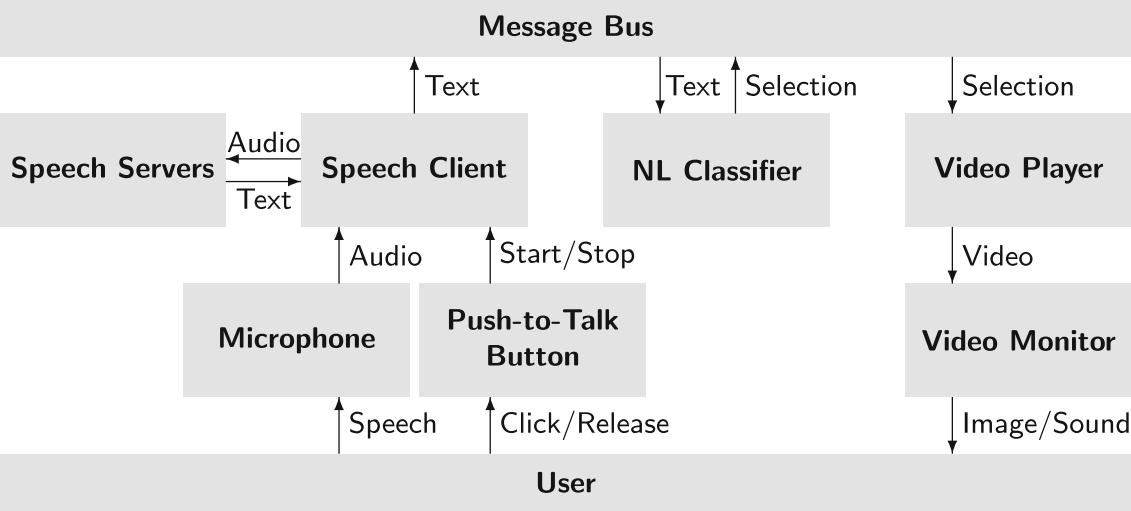
\includegraphics[width=\linewidth]{TraumDEtAl_DimensionsInTestimony_SystemArchitecture.png}
    \caption{Dimensions in Testimony - Systeem Architectuur \autocite{Traum2015}}
    \label{fig:DiTArchitecture}
\end{figure}

Spraakherkenning is de laatste jaren veel vooruit gegaan, dit komt omdat er meer data beschikbaar is, de algoritmes beter (deep neural networks) en de computers sneller zijn. Maar perfect zullen ze nooit zijn zegt \textcite{Hessen2020}. Dit is geen verassing aangezien mensen zelf vaak nog problemen hebben bij het verstaan van een andere. De meest voorkomende fouten van een ASR zijn herkenningsfouten. Deze kunnen ontstaan door slechte kwaliteit van de opname maar ook van de manier waarop woorden worden uitgesproken. De andere fouten ontstaan omdat ASR zijn vocabulaire niet uitgebreid genoeg is. Dit noemend we Out-of-vocabulary-fouten (OOV) \autocite{Hessen2020}.

Naast de ASR hebben we ook de natuurlijke taalverwerking (NLP). In 'Dimension in Testimony' maakten ze hiervoor gebruik van NCPEditor (Figuur \ref{fig:NPCEArchitecture}). De classifier in dit systeem berekent welke antwoorden op de ingegeven tekst kunnen gegeven worden door de taalmodellen van beide te vergelijken en de antwoorden te rangschikken. Zolang de ingegeven tekst een foutmarge lager dan 50\% blijft, zal het antwoord ongewijzigd blijven \autocite{Leuski2010}.

\begin{figure}[h]
    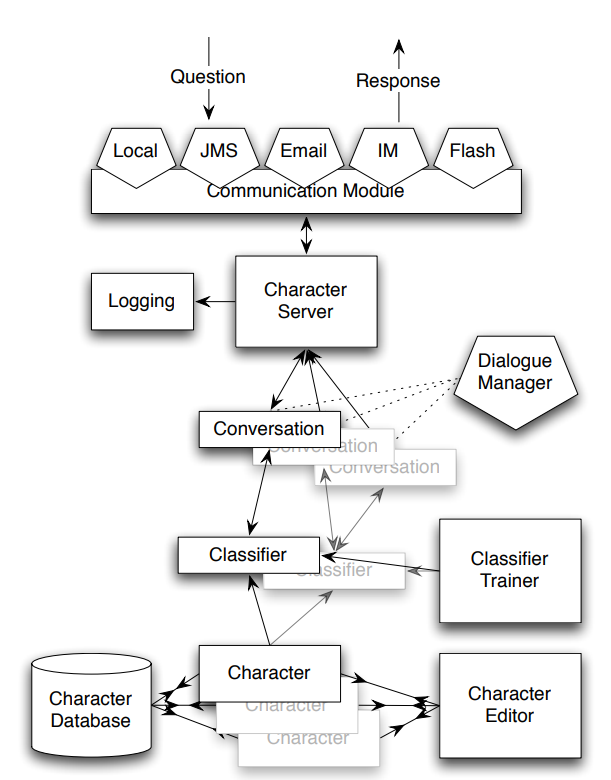
\includegraphics[width=\linewidth]{Traum&Leuski_NPCEditor_System architecture.png}
    \caption{NPCEditor - Systeem Architectuur \autocite{Leuski2010}}
    \label{fig:NPCEArchitecture}
\end{figure}

%Hier beschrijf je de \emph{state-of-the-art} rondom je gekozen onderzoeksdomein, d.w.z.\ een inleidende, doorlopende tekst over het onderzoeksdomein van je bachelorproef. Je steunt daarbij heel sterk op de professionele \emph{vakliteratuur}, en niet zozeer op populariserende teksten voor een breed publiek. Wat is de huidige stand van zaken in dit domein, en wat zijn nog eventuele open vragen (die misschien de aanleiding waren tot je onderzoeksvraag!)?
%
%Je mag de titel van deze sectie ook aanpassen (literatuurstudie, stand van zaken, enz.). Zijn er al gelijkaardige onderzoeken gevoerd? Wat concluderen ze? Wat is het verschil met jouw onderzoek?
%
%Verwijs bij elke introductie van een term of bewering over het domein naar de vakliteratuur, bijvoorbeeld~\autocite{Hykes2013}! Denk zeker goed na welke werken je refereert en waarom.
%
%Draag zorg voor correcte literatuurverwijzingen! Een bronvermelding hoort thuis \emph{binnen} de zin waar je je op die bron baseert, dus niet er buiten! Maak meteen een verwijzing als je gebruik maakt van een bron. Doe dit dus \emph{niet} aan het einde van een lange paragraaf. Baseer nooit teveel aansluitende tekst op eenzelfde bron.
%
%Als je informatie over bronnen verzamelt in JabRef, zorg er dan voor dat alle nodige info aanwezig is om de bron terug te vinden (zoals uitvoerig besproken in de lessen Research Methods).

% Voor literatuurverwijzingen zijn er twee belangrijke commando's:
% \autocite{KEY} => (Auteur, jaartal) Gebruik dit als de naam van de auteur
%   geen onderdeel is van de zin.
% \textcite{KEY} => Auteur (jaartal)  Gebruik dit als de auteursnaam wel een
%   functie heeft in de zin (bv. ``Uit onderzoek door Doll & Hill (1954) bleek
%   ...'')

%Je mag deze sectie nog verder onderverdelen in subsecties als dit de structuur van de tekst kan verduidelijken.

%---------- Methodologie ------------------------------------------------------
\section{Methodologie}%
\label{sec:methodologie}

Om te beginnen zal er worden samengezeten met het team van het zorglab. Zo kan worden neergeschreven wat de problemen zijn waar ze tegenaan lopen. Ook wordt besproken wat er verwacht wordt van een oplossing, hoe moet deze in zijn werk gaan? Op basis daarvan zal de literatuurstudie uitgebreid worden met onderzoek naar oplossingen die dit probleem kunnen verhelpen. Hieronder valt onder andere een onderzoek naar ASR. Er zal gekeken worden welke ASR's er al verkrijgbaar zijn en welke er in het Nederlands werken. Alleen een ASR hebben is niet genoeg om de immersie te behouden dus zal er ook worden gekeken naar hoe, aan de hand van de gegenereerde tekst, het volgende fragment kan getoond worden.

Wanneer er een uitgebreide literatuurstudie is uitgevoerd, zal de software die gevonden is op de proef gesteld worden. Hier wordt gekeken hoe correct de ASR's inkomende audio kunnen transcriberen. Dit wordt getest bij mensen zonder spraakaandoeningen als bij degene met een spraakaandoening zoals bijvoorbeeld stotteren. Daarnaast zal ook getest worden of er aan de hand van kernwoorden een juist fragment kan gekozen worden. Door de AI verschillende prompts te geven en te kijken of hij naar de juiste tijdsaanduiding in de video gaat.

Als laatste is het de bedoeling dat beide software samen in de context van het zorglab getest wordt.

%Hier beschrijf je hoe je van plan bent het onderzoek te voeren. Welke onderzoekstechniek ga je toepassen om elk van je onderzoeksvragen te beantwoorden? Gebruik je hiervoor literatuurstudie, interviews met belanghebbenden (bv.~voor requirements-analyse), experimenten, simulaties, vergelijkende studie, risico-analyse, PoC, \ldots?
%
%Valt je onderwerp onder één van de typische soorten bachelorproeven die besproken zijn in de lessen Research Methods (bv.\ vergelijkende studie of risico-analyse)? Zorg er dan ook voor dat we duidelijk de verschillende stappen terug vinden die we verwachten in dit soort onderzoek!
%
%Vermijd onderzoekstechnieken die geen objectieve, meetbare resultaten kunnen opleveren. Enquêtes, bijvoorbeeld, zijn voor een bachelorproef informatica meestal \textbf{niet geschikt}. De antwoorden zijn eerder meningen dan feiten en in de praktijk blijkt het ook bijzonder moeilijk om voldoende respondenten te vinden. Studenten die een enquête willen voeren, hebben meestal ook geen goede definitie van de populatie, waardoor ook niet kan aangetoond worden dat eventuele resultaten representatief zijn.
%
%Uit dit onderdeel moet duidelijk naar voor komen dat je bachelorproef ook technisch voldoen\-de diepgang zal bevatten. Het zou niet kloppen als een bachelorproef informatica ook door bv.\ een student marketing zou kunnen uitgevoerd worden.
%
%Je beschrijft ook al welke tools (hardware, software, diensten, \ldots) je denkt hiervoor te gebruiken of te ontwikkelen.
%
%Probeer ook een tijdschatting te maken. Hoe lang zal je met elke fase van je onderzoek bezig zijn en wat zijn de concrete \emph{deliverables} in elke fase?

%---------- Verwachte resultaten ----------------------------------------------
\section{Verwacht resultaat, conclusie}%
\label{sec:verwachte_resultaten}

Uit deze bachelorproef word verwacht dat er een oplossing op het immersie probleem gevonden wordt. Hiervoor zal de Spraakherkenning software gekozen worden die het beste resultaten geeft samen met een natuurlijke taalverwerking software. Het liefst zou deze al geïmplementeerd en wekende zijn in het zorglab. Als het niet zover komt dan zou er ten minste bestaan uit een goed uitgeschreven werking zodat de het kan geïmplementeerd worden in het zorglab.

%Hier beschrijf je welke resultaten je verwacht. Als je metingen en simulaties uitvoert, kan je hier al mock-ups maken van de grafieken samen met de verwachte conclusies. Benoem zeker al je assen en de onderdelen van de grafiek die je gaat gebruiken. Dit zorgt ervoor dat je concreet weet welk soort data je moet verzamelen en hoe je die moet meten.
%
%Wat heeft de doelgroep van je onderzoek aan het resultaat? Op welke manier zorgt jouw bachelorproef voor een meerwaarde?
%
%Hier beschrijf je wat je verwacht uit je onderzoek, met de motivatie waarom. Het is \textbf{niet} erg indien uit je onderzoek andere resultaten en conclusies vloeien dan dat je hier beschrijft: het is dan juist interessant om te onderzoeken waarom jouw hypothesen niet overeenkomen met de resultaten.

